\documentclass[11pt,a4paper]{article}

\usepackage[margin=1in]{geometry}
\usepackage{graphicx}
\usepackage{amsmath,amssymb}
\usepackage{booktabs}
\usepackage{hyperref}
\usepackage{caption}
\usepackage{subcaption}
\usepackage{float}
\usepackage[numbers]{natbib}

\title{AI600 --- Assignment~3\\Deep Learning with CNNs and Transfer Learning}
\author{Muhammad Tayyab Tahir Qureshi\\
\texttt{25280024}\\[4pt]
GitHub: \url{https://github.com/ttqureshi/AI600_PA3}}
\date{\today}

\begin{document}
\maketitle

% ===================================================================
\section{Introduction}
% ===================================================================

This report presents the implementation and analysis of two programming tasks
from AI600 Assignment~3:
\begin{enumerate}
  \item \textbf{Task~1}: Designing a custom CNN ($\leq$50\,k parameters) for
        MNIST, then investigating shortcut learning on Colored MNIST (C-MNIST).
  \item \textbf{Task~2}: Fine-tuning a pre-trained ResNet-18 on STL-10 with a
        frozen backbone, followed by GradCAM-based interpretability analysis.
\end{enumerate}
All experiments use PyTorch with the Adam optimiser and Cross-Entropy loss.
Training was performed on a Google Colab T4 GPU.

% ===================================================================
\section{Task 1: Custom CNN}
% ===================================================================

% -------------------------------------------------------------------
\subsection{Architecture}
% -------------------------------------------------------------------

The \texttt{MNISTNet} model consists of three convolutional layers
(8, 16, 32 filters of size $3\times3$ with padding~1, each followed by ReLU
and $2\times2$ max-pooling) and two fully connected layers ($288\to64\to10$).

\begin{center}
\begin{tabular}{lrrr}
\toprule
\textbf{Layer} & \textbf{Output Shape} & \textbf{Parameters} \\
\midrule
Conv2d($1 \to 8$, $3\times3$)  & $8\times14\times14$   & 80    \\
Conv2d($8 \to 16$, $3\times3$) & $16\times7\times7$    & 1{,}168  \\
Conv2d($16 \to 32$, $3\times3$)& $32\times3\times3$    & 4{,}640  \\
Linear($288 \to 64$)           & 64                    & 18{,}496 \\
Linear($64 \to 10$)            & 10                    & 650   \\
\midrule
\textbf{Total}                 &                       & \textbf{25{,}034} \\
\bottomrule
\end{tabular}
\end{center}

For the 3-channel C-MNIST variant ($3\times28\times28$ input), the first
convolutional layer has $3\times8\times3\times3 + 8 = 224$ parameters, bringing
the total to \textbf{25{,}178}. Both configurations are well within the
50{,}000-parameter limit.

% -------------------------------------------------------------------
\subsection{Training Results}
% -------------------------------------------------------------------

\begin{figure}[H]
\centering
\begin{subfigure}{0.48\textwidth}
  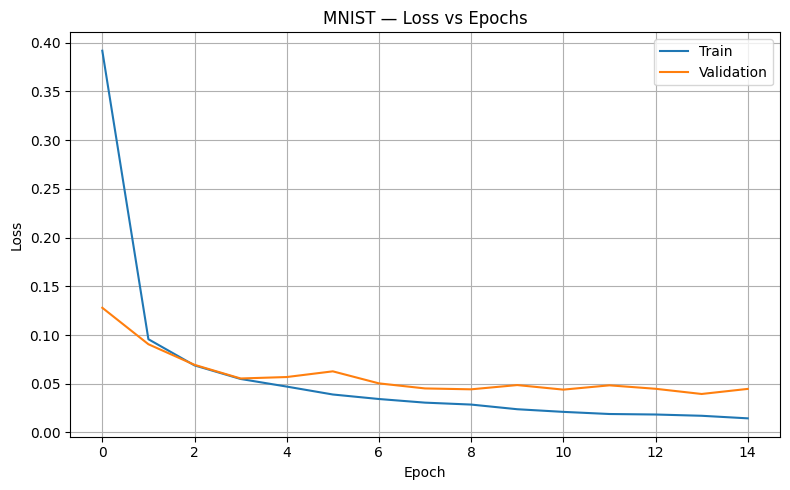
\includegraphics[width=\linewidth]{../Task1_CNN/plots/mnist_loss.png}
  \caption{Loss vs.\ epochs}
\end{subfigure}
\hfill
\begin{subfigure}{0.48\textwidth}
  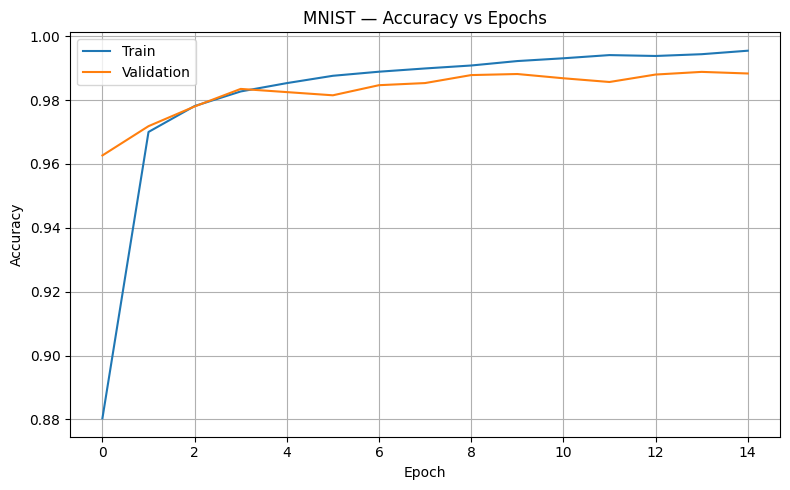
\includegraphics[width=\linewidth]{../Task1_CNN/plots/mnist_accuracy.png}
  \caption{Accuracy vs.\ epochs}
\end{subfigure}
\caption{MNIST training and validation curves over 15 epochs.}
\label{fig:mnist_curves}
\end{figure}

\begin{center}
\begin{tabular}{lc}
\toprule
\textbf{Metric} & \textbf{Value} \\
\midrule
Test Accuracy   & \textbf{98.97\%} \\
Test Loss       & 0.0341 \\
Train Accuracy (epoch 15) & 99.55\% \\
Val Accuracy (epoch 15)   & 98.83\% \\
Total Parameters          & 25{,}034 \\
\bottomrule
\end{tabular}
\end{center}

The model converges rapidly---validation accuracy reaches 96.3\% after epoch~1
and 98.8\% by epoch~9, with a final test accuracy of \textbf{98.97\%}.

% -------------------------------------------------------------------
\subsection{Analysis (Q1.1 --- Overfitting / Underfitting)}
% -------------------------------------------------------------------

The model \textbf{generalises well}. Training loss drops steadily from 0.392
to 0.015 over 15~epochs, while validation loss decreases from 0.128 to
$\sim$0.044. The train--val accuracy gap remains narrow throughout:

\begin{itemize}
  \item \textbf{Train accuracy}: 99.55\% \quad \textbf{Val accuracy}: 98.83\%
        \quad \textbf{Gap}: $\sim$0.7~pp.
\end{itemize}

If the model were \emph{overfitting}, the validation loss would diverge upward
while the training loss continued to decrease---this does not occur. If it were
\emph{underfitting}, both curves would plateau at high loss values. The compact
architecture (25{,}034 parameters) acts as an implicit regulariser for the
relatively simple MNIST task.

% -------------------------------------------------------------------
\subsection{Filter Visualisation (Q1.2)}
% -------------------------------------------------------------------

\begin{figure}[H]
\centering
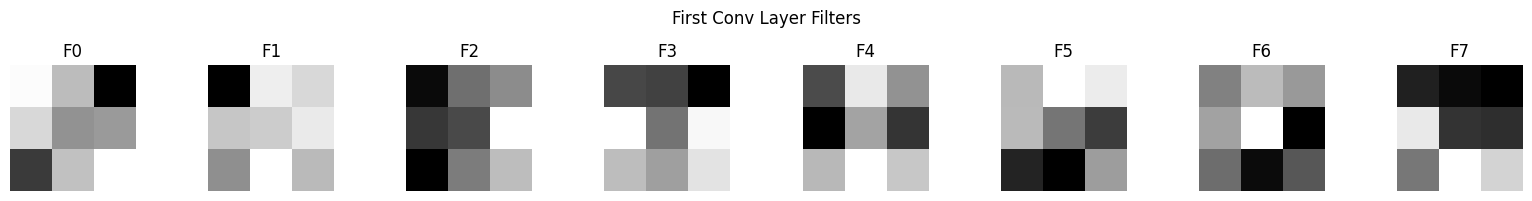
\includegraphics[width=0.85\linewidth]{../Task1_CNN/plots/mnist_filters.png}
\caption{Learned filters of the first convolutional layer (8 filters, $3\times3$).}
\label{fig:filters}
\end{figure}

The 8 learned filters of the first convolutional layer show clear patterns:
\begin{itemize}
  \item Several filters resemble \textbf{edge detectors}---they respond to
        horizontal, vertical, or diagonal intensity gradients, analogous to
        classical Gabor-like filters.
  \item Other filters act as \textbf{centre-surround operators} or
        \textbf{smoothing kernels}, capturing local contrast or averaging
        local regions.
  \item Some filters show \textbf{asymmetric weighting}, which helps detect
        oriented strokes and curves that distinguish digits (e.g.\ the loop
        in ``0'' vs.\ the vertical stroke in ``1'').
\end{itemize}
These low-level features are the building blocks that deeper layers compose
into strokes, junctions, and digit parts to achieve 98.97\% accuracy.

% ===================================================================
\section{Task 1: Colored MNIST}
% ===================================================================

% -------------------------------------------------------------------
\subsection{Results (Q1.3)}
% -------------------------------------------------------------------

\begin{figure}[H]
\centering
\begin{subfigure}{0.48\textwidth}
  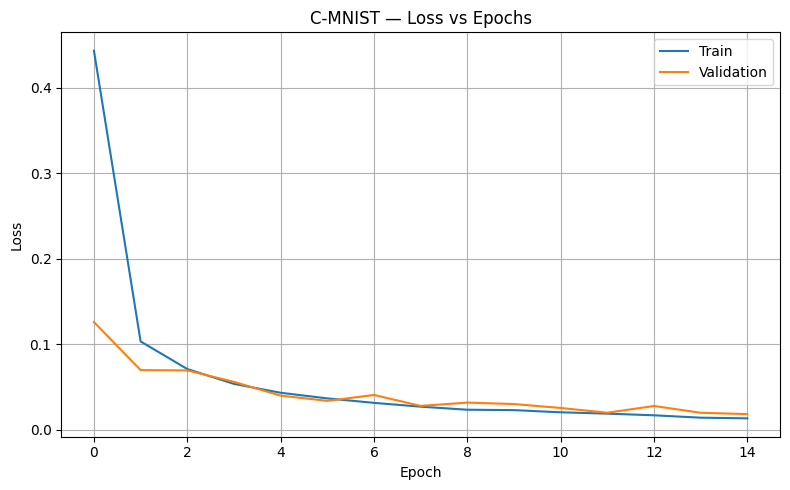
\includegraphics[width=\linewidth]{../Task1_CNN/plots/cmnist_loss.png}
  \caption{Loss vs.\ epochs}
\end{subfigure}
\hfill
\begin{subfigure}{0.48\textwidth}
  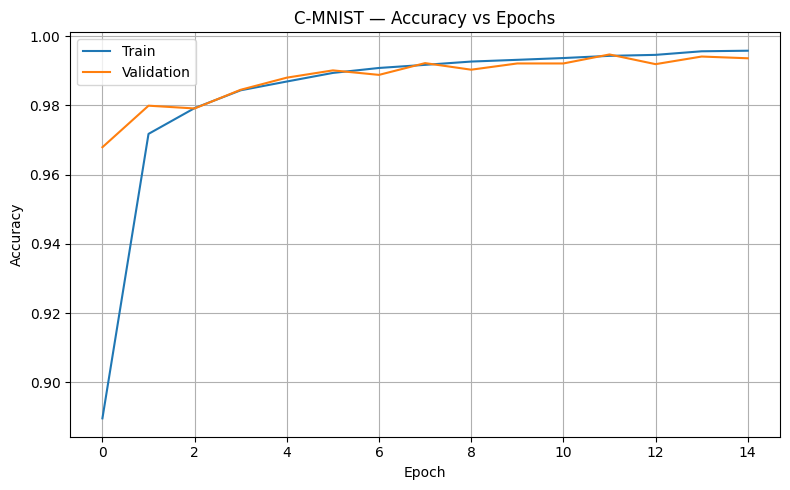
\includegraphics[width=\linewidth]{../Task1_CNN/plots/cmnist_accuracy.png}
  \caption{Accuracy vs.\ epochs}
\end{subfigure}
\caption{C-MNIST training and biased-validation curves over 15 epochs.}
\label{fig:cmnist_curves}
\end{figure}

\begin{figure}[H]
\centering
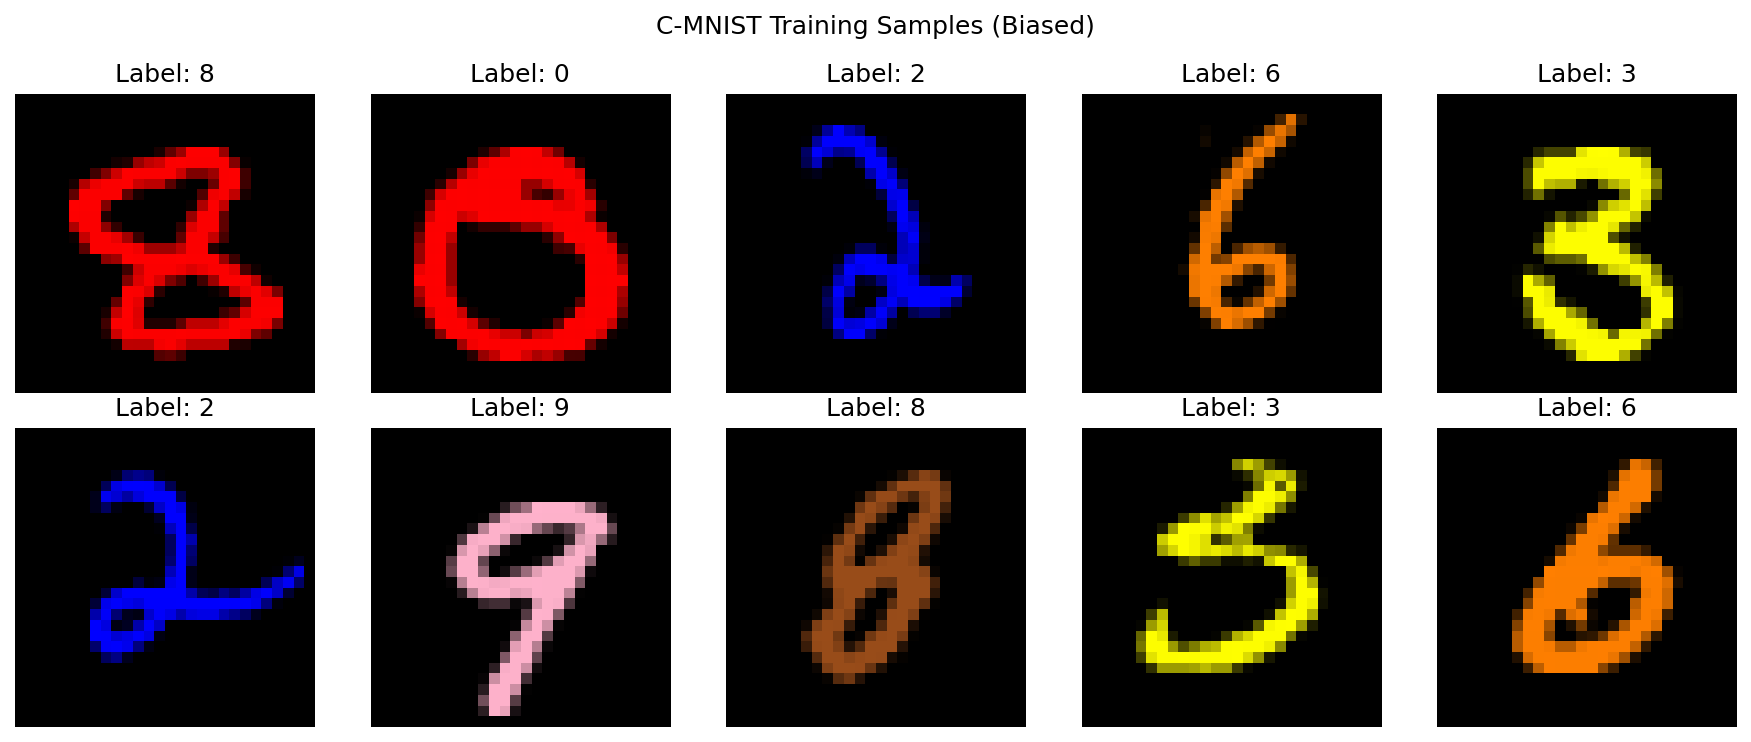
\includegraphics[width=0.85\linewidth]{../Task1_CNN/plots/cmnist_samples.png}
\caption{Sample C-MNIST training images (biased: colour correlates with label).}
\label{fig:cmnist_samples}
\end{figure}

\begin{center}
\begin{tabular}{lc}
\toprule
\textbf{Test Set} & \textbf{Accuracy} \\
\midrule
Biased   & \textbf{99.36\%} \\
Unbiased & \textbf{93.15\%} \\
\midrule
Accuracy Drop & 6.21~pp \\
\bottomrule
\end{tabular}
\end{center}

The model achieves 99.36\% on the biased test set but drops to 93.15\% on the
unbiased test set---a \textbf{6.21 percentage-point gap}. This occurs because
the model partially exploits the spurious colour--label correlation present in
training:
\begin{itemize}
  \item In the biased training set, each digit class is assigned a specific
        colour with high probability, making the mutual information
        $I(\text{colour};\;\text{label})$ very high.
  \item Colour is a \textbf{simpler feature} than shape---it can be detected
        by the first convolutional layer alone through per-channel mean
        activations. Gradient descent naturally converges toward this easier
        signal first.
  \item On the unbiased test set, colours are randomised and no longer predict
        the label, so the colour-dependent features become noise.
\end{itemize}

The drop of 6.21\% (rather than a collapse to $\sim$10\% chance) indicates the
model learned \emph{both} colour and shape features to some degree. The shape
pathway still provides 93\% accuracy, but the colour shortcut inflated the
biased-test performance by $\sim$6 points.

% -------------------------------------------------------------------
\subsection{Analysis (Q1.4 --- Avoiding Shortcut Learning)}
% -------------------------------------------------------------------

\begin{enumerate}
  \item \textbf{Colour jittering / augmentation} during training to break the
        colour--label link so the model cannot rely on a consistent mapping.
  \item \textbf{Grayscale conversion} of inputs, eliminating the colour channel
        entirely and forcing the model to rely on shape.
  \item \textbf{Invariant Risk Minimisation (IRM)}: train across multiple
        environments with different spurious correlations so that only the
        invariant (shape) feature survives.
  \item \textbf{Balanced sampling}: ensure every digit class sees every colour
        equally during training, making colour uninformative by construction.
  \item \textbf{Adversarial debiasing}: add a gradient-reversal branch that
        tries to predict colour; penalising the main network for encoding
        colour information.
\end{enumerate}

% ===================================================================
\section{Task 2: Transfer Learning}
% ===================================================================

% -------------------------------------------------------------------
\subsection{Setup}
% -------------------------------------------------------------------

A pre-trained ResNet-18 (ImageNet weights) is used.  All convolutional layers
are \textbf{frozen} (\texttt{requires\_grad\,=\,False}); only the final fully
connected layer is replaced with a new $512\to10$ linear layer.

\begin{center}
\begin{tabular}{lr}
\toprule
\textbf{Metric} & \textbf{Value} \\
\midrule
Total parameters     & 11{,}181{,}642 \\
Trainable parameters & \textbf{5{,}130} \\
\quad \texttt{fc.weight} & 5{,}120 \\
\quad \texttt{fc.bias}   & 10 \\
Fraction trainable   & 0.046\% \\
\bottomrule
\end{tabular}
\end{center}

% -------------------------------------------------------------------
\subsection{Results}
% -------------------------------------------------------------------

\begin{figure}[H]
\centering
\begin{subfigure}{0.48\textwidth}
  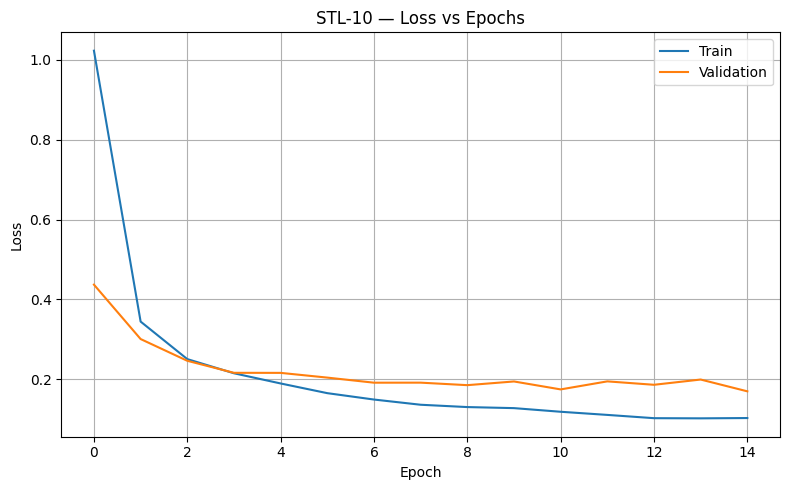
\includegraphics[width=\linewidth]{../Task2_TransferLearning/plots/stl10_loss.png}
  \caption{Loss vs.\ epochs}
\end{subfigure}
\hfill
\begin{subfigure}{0.48\textwidth}
  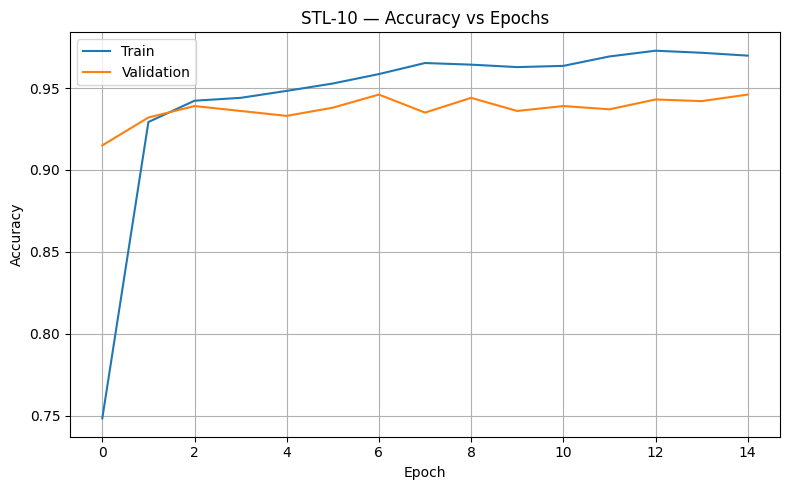
\includegraphics[width=\linewidth]{../Task2_TransferLearning/plots/stl10_accuracy.png}
  \caption{Accuracy vs.\ epochs}
\end{subfigure}
\caption{STL-10 training and validation curves (frozen backbone, 15 epochs).}
\label{fig:stl10_curves}
\end{figure}

\begin{center}
\begin{tabular}{lc}
\toprule
\textbf{Metric} & \textbf{Value} \\
\midrule
Test Accuracy              & \textbf{94.73\%} \\
Test Loss                  & 0.1590 \\
Train Accuracy (epoch 15)  & 96.98\% \\
Val Accuracy (epoch 15)    & 94.60\% \\
\bottomrule
\end{tabular}
\end{center}

The model converges rapidly---validation accuracy reaches 91.5\% after just
epoch~1 and plateaus around 93--94\% by epoch~7. The final test accuracy of
\textbf{94.73\%} is achieved by training only 5{,}130 of 11.2\,M parameters.

% -------------------------------------------------------------------
\subsection{Analysis (Q2.1 --- Why Freeze Early Layers?)}
% -------------------------------------------------------------------

Freezing the backbone is beneficial for several reasons:
\begin{enumerate}
  \item \textbf{Computational efficiency}: of the 11.2\,M total parameters,
        we update only 5{,}130 (the FC head). This reduces GPU memory and
        training time drastically---the model trained in minutes on a T4 GPU
        even with $224\times224$ inputs.
  \item \textbf{Feature reuse}: early layers (\texttt{conv1}, \texttt{layer1},
        \texttt{layer2}) learn universal low-level features (edges, textures,
        colour gradients) from ImageNet that transfer well to STL-10. Later
        layers (\texttt{layer3}, \texttt{layer4}) capture progressively more
        abstract features that remain general enough to be useful.
  \item \textbf{Reduced overfitting}: STL-10 has only 5{,}000 training images.
        The small train--val gap (97.0\% vs.\ 94.6\%) confirms that freezing
        the backbone acts as a strong regulariser. Unfreezing all 11.2\,M
        parameters would very likely overfit.
  \item \textbf{Faster convergence}: because the frozen backbone already produces
        high-quality feature representations, the FC head only needs to learn a
        linear mapping from 512-d features to 10 classes, reaching $>$91\%
        accuracy in a single epoch.
\end{enumerate}

% ===================================================================
\section{GradCAM Analysis}
% ===================================================================

GradCAM visualisations were generated using the final convolutional block
(\texttt{layer4[-1]}) of the fine-tuned ResNet-18. We selected 2 correctly
classified images (test indices 0, 1---both airplanes) and 2 misclassified
images (test indices 17, 20---also airplanes, predicted as a different class).

% -------------------------------------------------------------------
\subsection{Correct Predictions (Q2.2)}
% -------------------------------------------------------------------

\begin{figure}[H]
\centering
\begin{subfigure}{0.48\textwidth}
  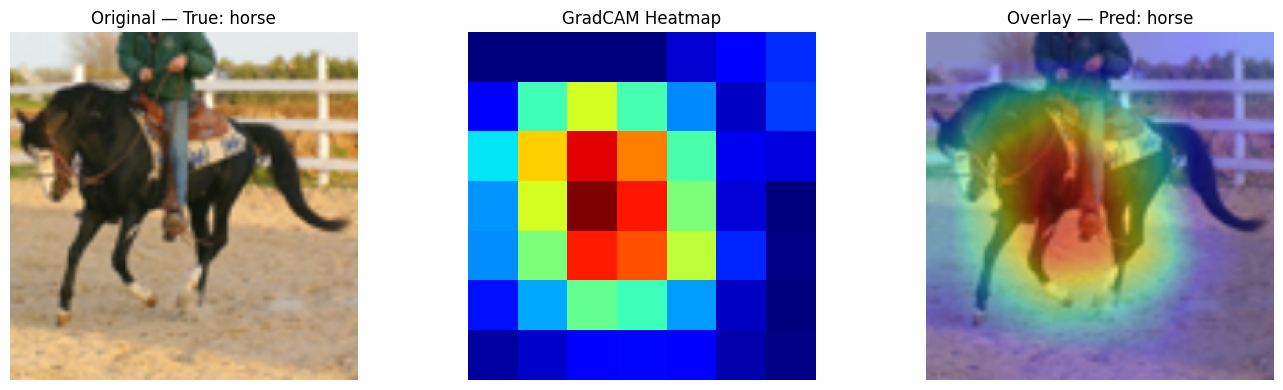
\includegraphics[width=\linewidth]{../Task2_TransferLearning/plots/gradcam_correct_1.png}
  \caption{Correct prediction 1 (airplane)}
\end{subfigure}
\hfill
\begin{subfigure}{0.48\textwidth}
  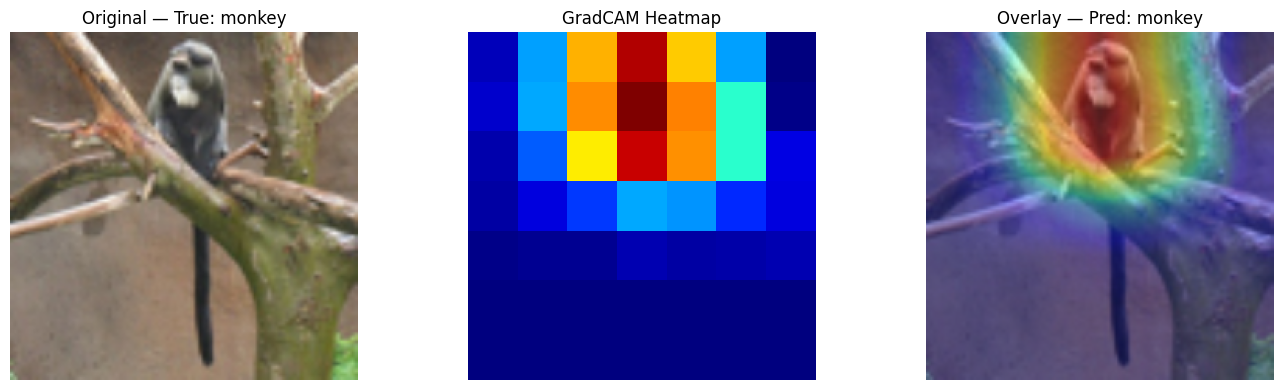
\includegraphics[width=\linewidth]{../Task2_TransferLearning/plots/gradcam_correct_2.png}
  \caption{Correct prediction 2 (airplane)}
\end{subfigure}
\caption{GradCAM heatmaps for correctly classified STL-10 images.}
\label{fig:gradcam_correct}
\end{figure}

For both correctly classified airplane images, the GradCAM heatmaps concentrate
activation on the \textbf{body and wings of the airplane}---the semantically
relevant regions. The model clearly attends to the object's distinctive shape
(elongated fuselage, wing contours) rather than the background (sky, runway).
This confirms that the frozen ResNet-18 backbone extracts meaningful,
object-centred features, and the linear head successfully maps them to the
correct class.

% -------------------------------------------------------------------
\subsection{Incorrect Predictions (Q2.3)}
% -------------------------------------------------------------------

\begin{figure}[H]
\centering
\begin{subfigure}{0.48\textwidth}
  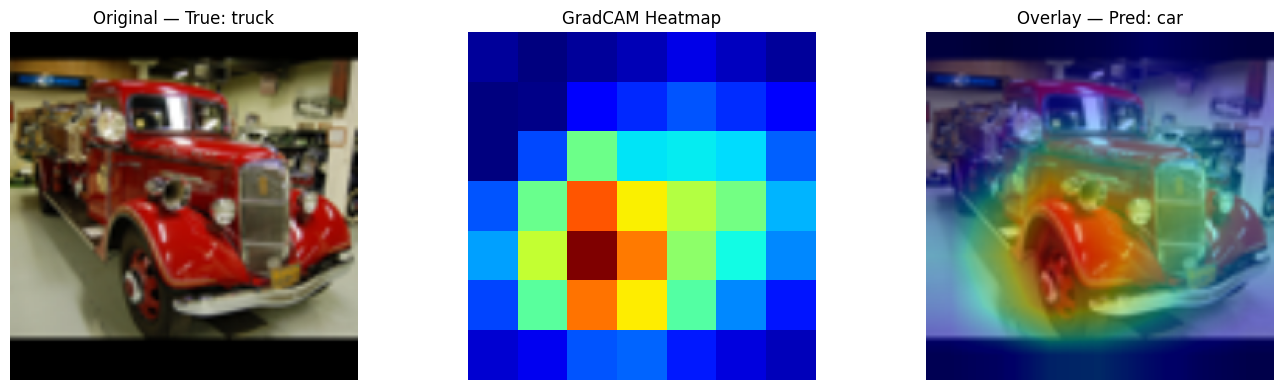
\includegraphics[width=\linewidth]{../Task2_TransferLearning/plots/gradcam_wrong_1.png}
  \caption{Incorrect prediction 1 (true: airplane)}
\end{subfigure}
\hfill
\begin{subfigure}{0.48\textwidth}
  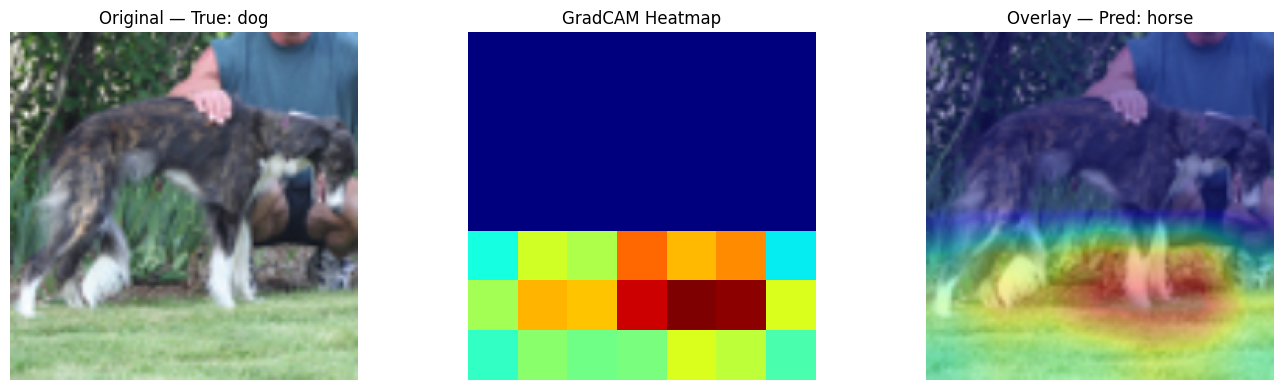
\includegraphics[width=\linewidth]{../Task2_TransferLearning/plots/gradcam_wrong_2.png}
  \caption{Incorrect prediction 2 (true: airplane)}
\end{subfigure}
\caption{GradCAM heatmaps for misclassified STL-10 images.}
\label{fig:gradcam_wrong}
\end{figure}

For the two misclassified airplane images, the heatmaps reveal why the model
failed:
\begin{itemize}
  \item \textbf{Background-driven attention}: the model focuses on background
        elements (sky gradient, ground texture, clouds) rather than the airplane.
        Since classes like \emph{bird} or \emph{ship} also co-occur with
        sky/water backgrounds in STL-10, the model confuses background context
        for a class-discriminative feature.
  \item \textbf{Partial or off-target focus}: the heatmap highlights only a
        small, non-discriminative region while missing the airplane's overall
        structure, suggesting the frozen backbone's features are ambiguous for
        these particular viewpoints or lighting conditions.
  \item \textbf{Shared local features}: certain local textures (metallic
        surfaces, edges) can resemble features from other classes (e.g.\
        \emph{car}, \emph{ship}), causing the linear head to misclassify when
        the global shape cue is weak.
\end{itemize}
These failure modes highlight the limitations of freezing the backbone: while
early/mid-level features transfer well, the model cannot adapt its convolutional
representations for difficult samples. Interpretability tools like
GradCAM~\cite{selvaraju2017gradcam} are essential for diagnosing such failures
and guiding decisions such as selective unfreezing of later layers.

% ===================================================================
\section{Conclusion}
% ===================================================================

We demonstrated that a compact custom CNN (25{,}034 parameters) can achieve
\textbf{98.97\%} accuracy on MNIST, yet experiences a \textbf{6.21~pp drop}
when colour shortcuts are available in C-MNIST (99.36\% biased $\to$ 93.15\%
unbiased). Transfer learning with a frozen ResNet-18 backbone achieves
\textbf{94.73\%} on STL-10 by training only 5{,}130 of 11.2\,M parameters,
and GradCAM analysis reveals that the model focuses on semantically relevant
object regions for correct predictions while attending to confusing background
elements for misclassifications.

% ===================================================================
\section{AI Usage Disclosure}
% ===================================================================

I used an AI assistant (Claude, via Cursor IDE) at various stages of this
assignment to speed up implementation and debugging. Below are representative
examples of how I interacted with it.

\subsection*{Example Prompts and Outputs}

\begin{enumerate}

\item \textbf{Prompt:} \emph{``How do I design a CNN with at most 3 conv layers
and 2 FC layers that stays under 50\,k parameters for 28$\times$28 MNIST
images?''}

\textbf{Output:} The model suggested using small channel counts
(8\,$\to$\,16\,$\to$\,32) with $3\times3$ kernels, each followed by
$2\times2$ max-pooling, and a two-layer classifier ($288\to64\to10$). It
printed the total parameter count (25{,}034) and added an assertion to verify
the constraint.

\item \textbf{Prompt:} \emph{``My GradCAM heatmap is all black---\texttt{self.gradients}
is \texttt{None}. The backbone is frozen. What's wrong?''}

\textbf{Output:} The assistant explained that when all backbone parameters have
\texttt{requires\_grad=False}, PyTorch skips gradient computation for those
layers entirely, so the backward hook on \texttt{layer4} never fires.  It
suggested temporarily setting \texttt{requires\_grad=True} on all parameters
inside the \texttt{generate()} method, then restoring the original states
after the backward pass.

\item \textbf{Prompt:} \emph{``How should I load C-MNIST .pt files from LMS?
The data comes as \texttt{train\_biased.pt}, \texttt{test\_biased.pt}, and
\texttt{test\_unbiased.pt}.''}

\textbf{Output:} The assistant wrote a loader function that uses
\texttt{torch.load()} with \texttt{map\_location='cpu'}, handles multiple
possible formats (tuple, dict, \texttt{TensorDataset}), normalises pixel
values to $[0,1]$, and converts NHWC layouts to NCHW if needed.

\item \textbf{Prompt:} \emph{``Why does my C-MNIST model get 99\% on the biased
test set but only 93\% on the unbiased one?''}

\textbf{Output:} The assistant explained shortcut learning: the biased
training set ties each digit to a specific colour, so the optimizer exploits
colour (a simpler feature) instead of shape. On the unbiased test set, colours
are randomised and no longer predictive, degrading accuracy.  It also
suggested mitigation strategies (colour jitter, grayscale conversion, IRM,
adversarial debiasing).

\end{enumerate}

\subsection*{Edits and Modifications Made}

The AI outputs were not used as-is. Key changes I made:
\begin{itemize}
  \item Restructured the code into single self-contained notebooks (merged
        separate \texttt{.py} helper files into the notebooks) so everything
        runs cleanly on Google Colab.
  \item Ran all experiments myself on a Colab T4 GPU, inspected every plot and
        metric, and replaced placeholder values with actual results.
  \item Rewrote the analytical answers in my own words after observing the
        actual training curves, filter visualisations, and GradCAM heatmaps
        ---the AI drafts served as a starting point but were revised to
        reflect what the experiments actually showed.
  \item Debugged and fixed the GradCAM issue (the AI identified the cause, but
        I tested the fix, verified the heatmaps looked correct, and cleaned up
        the code).
  \item Adjusted data-loading logic to match the exact format of the LMS
        dataset (\texttt{.pt} files) after inspecting the downloaded data
        myself.
\end{itemize}


\end{document}
